\chapter{LArIAT: Liquid Argon In A Testbeam}\label{sec:experimentDescription}
\section{LArIAT \& the Intensity Frontier}
\section{The Particles Path to LArIAT}

LArIAT's home at Fermilab is the Fermilab Test Beam Facility (FTBF), where the experiment 
characterizes a beam of charge particles downstream from the Meson Center beam line. 

LArIAT's particles history begins in the Fermilab accelerator complex with a beam of protons. 
The process of protons acceleration develops in gradual stages, see picture \ref{fig:Accelerator}: gaseous hydrogen is ionized in order to form H$^{-}$ ions; these ions are boosted to 750 keV by a Cockroft-Walton accelerator and injected to the Linac linear accelerator that increases their energy up to 400 MeV; then, H$^{-}$ ions pass through a carbon foil and lose the two electrons; the resulting protons are then injected into a rapid cycling synchrotron, called Booster; at this stage protons reach 8 GeV of energy and are compacted into bunches; the next stage of acceleration is the Main Injector, a synchrotron which accelerates the bunches up to 120 GeV; in the Main Injector, several bunches are merged into one and used for the injection in the last stage.


The Fermilab accelerator complex works in supercycles of roughly 60 seconds in duration. The beam is then split by electrostatic septa and delivered at different experimental halls all over the lab. A 120~GeV$/c$ primary proton beam with variable intensity is extracted in four-second ``spills" and sent to the Meson Center beam line. Here, this primary beam is focused onto a tungsten target to create LArIAT's secondary beam. The composition of the secondary particle beam is mainly positive pions. For the LArIAT data considered in this work the secondary beam peak momentum was fixed at 64~GeV$/c$, although the beam is tunable in momentum between 8-80\,GeV$/c$; this was deemed a secondary beamline configuration which allowed a stable beam operation of the FTBF.
The beam of pions impinges then on a copper target within a steel collimator inside the LArIAT experimental hall (MC7) to create LArIAT tertiary beam, whose geometry in MC7 has been optimized for LArIAT (shown in  Fig.~\ref{fig:tert-layout}).   The steel collimator selects particles produced with a $13^\circ$ production angle at the target down the beamline.  The particles are then bend by  $~10^\circ$  through a pair of dipole magnets.  Tuning the magnets field intensity results in a range of particle momenta from 0.2 to 1.4~GeV/c.
The tertiary beam composition counts mostly pions and protons with a small fraction of electrons, muons, and kaons present as well. It is the job of the LArIAT beamline detectors to select the particles polarity,  to perform particle identification (beamPID) and to measure the momentum of the tertiary beam particles before they get to the LArTPC. The LArIAT detectors are described in the following paragraphs.  

%\begin{comment}     
\begin{figure}
  \centering  	
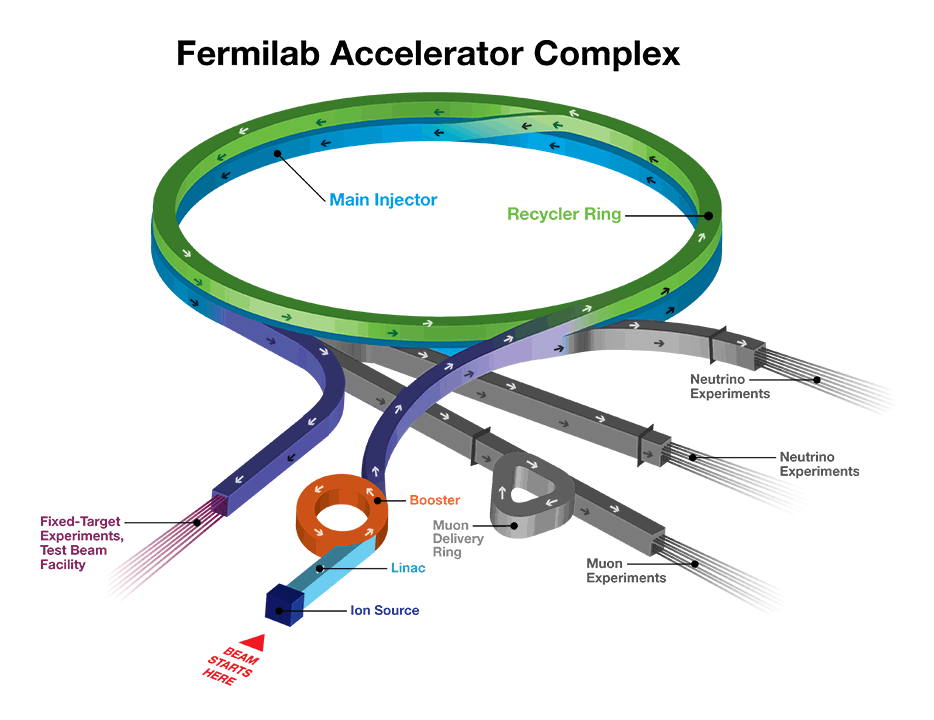
\includegraphics[width=\textwidth,height=\textheight,keepaspectratio]{Chapter-2/Images/AcceleratorFNAL.png}
\label{fig:Accelerator}
\caption{Layout of Fermilab Acellerator complex.}
\end{figure}

%\begin{comment}     
\begin{figure}
  \centering  	
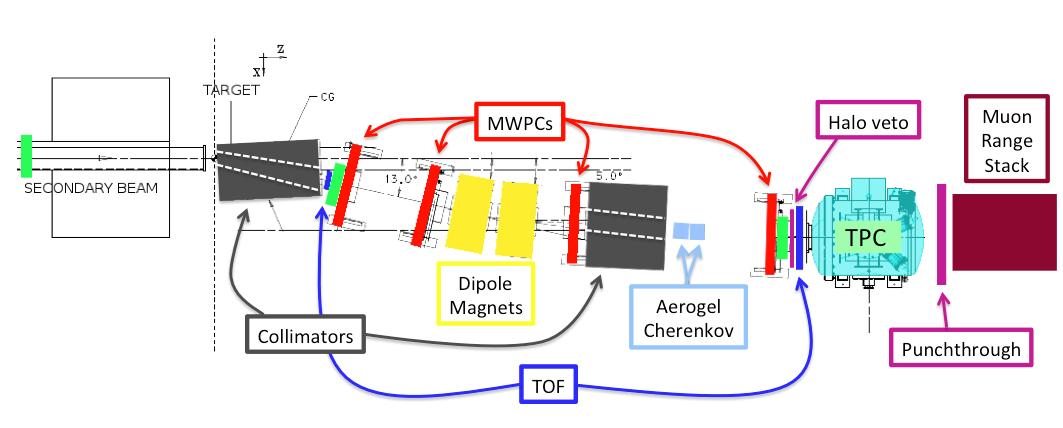
\includegraphics[width=\textwidth,height=\textheight,keepaspectratio]{Chapter-2/Images/Tertiary.png}
\label{fig:tert-layout}
\caption{Birds eye view of the LArIAT tertiary beamline. In grey: upstream and downstream collimators; in yellow: bending magnets in yellow; in red: wire chambers; in blue: time of flight; in green: liquid argon TPC volume; in maroon: muon range statck.}
\end{figure}


%%%%%%%%%%%%%%%%%%%%%%%%%%%%%%%%%%%%%%%%%%%%%%%%%%%%%%%%%%%%
\section{LArIAT Tertiary Beam Instrumentation}\label{sec:Instrumentation}

%%%%%%%%%%%%%%%%%%%%%%%%%%%%%%%%%%%%%%%%%%%%%%%%%%%%%%%%%%%%
The instrumentation of  LArIAT tertiary beam and the TPC components have changed several times during the three years of LArIAT data taking. The following paragraphs describe the components operational during the data taking period relevant to the hadron cross section measurements (a.k.a. Run II).

The components of the tertiary beamline instrumentation key for the hadron cross section analyses are the target and collimators system, the two bending magnets (in a similar configuration used for the  MINERvA T-977 test beam calibration~\cite{MinervaTestbeam}) a set of four wire chambers (WCs) and two time-of-flight scintillating paddles (TOF) and, of course, the LArTPC.  The magnets determine the polarity of the particles in the tertiary beam; the combination of magnets and wire chambers determine the particles momentum, which is used to determine the particle species in conjunction with the TOF.
A muon range stack downstream from the TPC and two sets of cosmic paddles configured as a telescope surrounding the TPC are also used for calibration purposes.


\subsection{Bending Magnets}\label{sec:Magnets}
%%%%%%%%%%%%%%%%%%%%%%%%%%%%%%%%%%%%%%%%%%%%%%%%%%%%%%%%%%%%
LArIAT uses a pair of identical Fermilab type ``NDB" electromagnets, recycled from the Tevatron's anti-proton ring \textcolor{red}{CITE CDF?}. 
The magnets are a fundamental piece of the LArIAT beamline as they are used in all the three tasks of the LArIAT beamline: the sign of the current in the magnet provide the selection of either positively or negatively charged particles, the value of the magnetic field is used in the momentum determination and the subsequent particle identification. 

We describe here the characteristics and response of one magnet. We expect the second one have a similar response, being identical in shape and with a similar history. The magnet aperture measures the gap dimensions to be 14.224~cm of height, 31.75~cm width, and  46.67~cm length.  The wire chambers aperture ($\sim$12.5~cm) is smaller than the magnet aperture, thus, only the central part of the magnet gap is utilized. The field is extremely uniform over this limited aperture and was measured with two Hall probes, both calibrated with nuclear magnetic resonance probes. The probes measured the excitation curve shown in Figure~\ref{fig:magnet_excitation}. 

\begin{figure}[!h]
\begin{centering}
\vspace{-0.3cm}
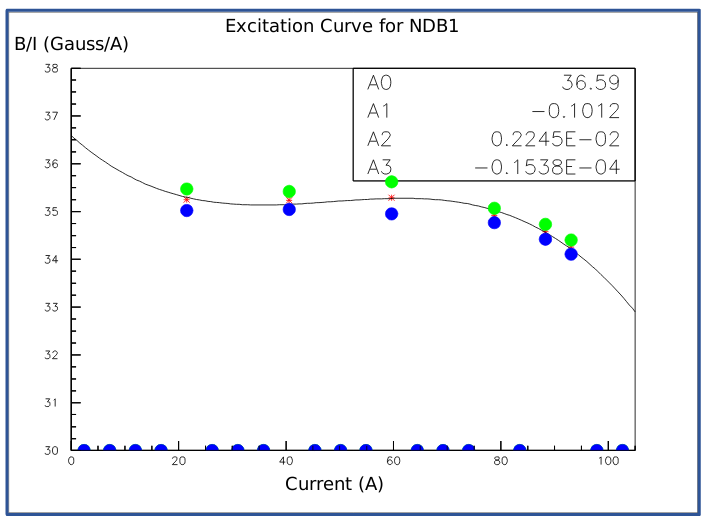
\includegraphics[height=3.0in]{Chapter-2/Images/ExcitationCurves.png}
\caption{
{ Magnetic field over current as a function of the current, for one NDB magnet (excitation curve). The data was collected using two Hall probes (blue and green). We fit the readings with a cubic function (black) to average of measurements (red) given in the legend.}
}
\label{fig:magnet_excitation}
\end{centering}
\end{figure}

The current being passed through the magnets at a given time is identical in both magnets. For Run II period, the current settings explored were 60A (B $\sim$0.21 T) and 100A (B $\sim$0.35 T) in both polarities. 
Albeit advantageous to enrich the tertiary beam composition with high mass particles such as kaons, we never pushed the magnets current over 100 A, not to incur in overheating.  During operation, we operated a air and water cooling system on the magnets and we remotely monitored the magnets temperature.
 





\section{In the Cryostat}

\subsection{TPC: Charge Collection}\label{sec:TPC}
\subsection{TPC: Light Collection System}
\subsection{Cryogenics and Purity Control}
\subsection{TPC: Electric Field Measurement}
\section{Trigger and DAQ}
\section{Control Systems}

\begin{comment}



%%%%%%%%%%%%%%%%%%%%%%%%%%%%%%%%%%%%%%%%%%%%%%%%%%%%%%%%%%%%
\subsubsection{Time-of-Flight System}\label{sec:TOF}
%%%%%%%%%%%%%%%%%%%%%%%%%%%%%%%%%%%%%%%%%%%%%%%%%%%%%%%%%%%%

The LArIAT time-of-flight (TOF) detector system consists broadly of two scintillator paddles, which bracket the beamline and are shown in blue in Figure~\ref{fig:tert-layout}. The exact details of the of the TOF system were changed between Run-II and Run-III to allow for better performance and timing resolution.

\paragraph{\textbf{TOF System for Run-I and Run-II:}}
The upstream paddle, shown in Figure \ref{}, has a relatively small active area (10~cm x 6~cm ) and was chosen to be a relatively thin piece of scintillator to minimize any impact on the momentum of the particles coming from the target. Light guides were mounted on all four edges which lead to two \textit{insert PMT type} PMTs mounted on the beam left side. The downstream paddle, shown in Figure \ref{fig:TOFSystemRunIandII}, was chosen to have a slightly larger area (14~cm x 14~cm) and had two \textit{insert PMT type} PMTs which were read out on opposite ends of the paddle.

\begin{figure}[!h]
\begin{centering}
\vspace{-0.3cm}
%\includegraphics[height=2.3in]{figures/tofdelay.png}
\caption{
{\scriptsize \sf Pictures of the TOF system as was deployed during Run-I and Run-II data taking. The left image is of the upstream TOF paddle and the right image is of the downstream TOF paddle }
}
\label{fig:TOFSystemRunIandII}
\end{centering}
\end{figure}


%The active area of the upstream paddle is relatively small ( 10~cm x 6~cm ) and that of the downstream paddle is somewhat larger ( 14~cmx 14~cm ). Lightguides are mounted on all four edges of each paddle. In the first two LARIAT production runs, each of the paddles was read out by two (xxkxkxkxk) photomultiplier tubes (PMTs), The long axis of the downstream paddle was directed horizontally and read out at either end. The upstream paddle was rotated by 45 degrees with respect to the horizontal and its two PMTs were mounted to the left side. In run 3, four more PMTs were added to the system. The upstream paddle was read out with the original set of PMTs and the downstream paddle with four 2" Hamamatsu PMTs (R-1828) inherited from the muon g-2 experiment(E821) at BNL.

During data-taking cycles, signals from the TOF PMTs were sampled at 1 GHz
with a CAEN 1751 digitizer and 12 bit samples were stored in a circular memory buffer. In response to an experimental trigger, a 28.7 $\mu$ second window of samples, starting approximately 8.4 $\mu$sec before the trigger, was written to the
output. The amplitude of the TOF signals was typically 200 mV in the upstream TOF PMTs but only 50 mV in those of the downstream counter. The signals have a rise time (10-90\%) of 4 ns and a full width, half-maximum of 9 ns. The rate in the upstream counter was typically 15 kHz and much less, 400 Hz in the downstream counter.

Because the shape of signals from each TOF PMT was highly uniform, the time of the pulses was determined using an oversampled template derived from the data itself. The DC offset (pulse pedestal) is taken from samples far from the pulse, The template is stretched vertically to match the pedestal-subtracted pulse amplitude and moved horizontally to match the time. The pulse time-pickoff resolution is better than 100 ps and relative amplitude resolution is better than x\%. Since the average rate of pulses incident on the ToF system is modest, pulse pile up is not a significant problem. Given the uniform width of the pulses produced by any given PMT (sigma of 400 ps), the pulse width can be used to flag events where two pulses overlap closely in time. Simulations indicate that for pulses as close as 4 ns, a well-chosen pulse width cut is 90\% efficient.

To determine the particles' time of arrival, pulse times from the multiple PMTs mounted on each paddle had to be combined. During Run-I and II, with two PMTs mounted on each paddle, a simple average was used. In the case of the downstream paddle, with PMTs mounted at opposite ends, the average corrected for the fact that transit time to the two PMTs depended on the particle's point of impact on the scintillator. A plot of the time of arrival {\it difference} between the two downstream PMTs vs the longitudinal impact point, made with the help of track stubs from the wire chamber system, is shown in Fig.~\ref{fig:tofdelay}. As expected, the time difference
changes systematically across the face of the scintillator.

\begin{figure}[!h]
\begin{centering}
\vspace{-0.3cm}
%\includegraphics[height=2.3in]{figures/tofdelay.png}
\caption{
{\scriptsize \sf $\Delta-t$ between times registered on two downstream paddles.}
}
\label{fig:tofdelay}
\end{centering}
\end{figure}

Taking the average minimizes ToF errors arising from optical path differences in the scintillator, However, even for a set of particles which pass through a single small area of the paddle, the times of pulses registered in the two PMTs are still spread by approximately 300~ps, an uncertainty which is probably caused by transit time jitter in the PMTs themselves. This jitter is evident in both the upstream and downstream detectors.

Although climate-control in the LArIAT experiment hall is fairly primitive, there is little sign of systematic timing drift over longer periods. The average time differences between pairs of PMTs reading out the same scintillator varied by no more than 150~ps over the 3-4 months of a data-taking period.


%%%%%%%%%%%%%%%%%%%%%%%%%%%%%%%%%%%%%%%%%%%%%%%%%%%%%%%%%%%%

%%%%%%%%%%%%%%%%%%%%%%%%%%%%%%%%%%%%%%%%%%%%%%%%%%%%%%%%%%%%
\subsubsection{Multi-Wire Proportional Chambers}\label{sec:MWPC}
%%%%%%%%%%%%%%%%%%%%%%%%%%%%%%%%%%%%%%%%%%%%%%%%%%%%%%%%%%%%
The wire chambers are based on the Fenker Chambers~\cite{Fenker} long in use at Fermilab.  The chambers have been upgraded by adding additional grounding to improve the signal to noise in the electronic readout.  The chambers, shown in Figure~\ref{fig:wirechamber}, have an effective aperture of 128~mm in both horizontal and vertical distances.  The wires are spaced at 1~mm, with 128 wires in each view.  In a test beam, the chambers have typical efficiencies of 98\% to 99\%. The gas used is 85\% Argon + 15\% isobutane.  The wire chambers typically operate between 2400 and 2500 volts.

\begin{figure}[!h]
\begin{centering}
\vspace{-0.3cm}
%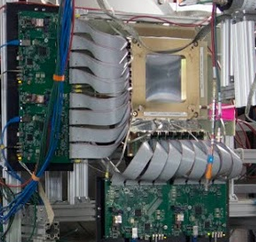
\includegraphics[height=2.3in]{figures/WireChamber.png}
\caption{
{\scriptsize \sf Image of one of the wire chambers used in the LArIAT tertiary beamline.}
}
\label{fig:wirechamber}
\end{centering}
\end{figure}

The front end amplifier/discriminator uses the ASDQ chip~\cite{ASDQchip}. Two of the ASDQ chips are mounted on a mother board that is plugged into the chamber.  Short flat cables are used to connect these ASDQ mother board to a new, multi-hit TDC~\cite{Sten}. This TDC provides a (maskable) fast OR output that can be used in a first level trigger. 

This TDC can accept multiple hits per wire with a time resolution of 1.18~ns/bin.  The TDCs can accept 2 edges per 9~ns.  The maximum event rate that can be accepted by the chamber system is of the order of one megahertz.  These limitations are clearly not an issue for the LArIAT beamline where the rates and timing resolution required are much less stringent than this.  There is enough memory on the TDC board to buffer a full spill of data (up to about 100 events/spill).  As in this application the spills occur only once per minute, there is ample time to read out the whole spill through a controller specially designed to support these TDCs.  Power and data flow to and from the controller to the TDCs and from the controller to the rest of the DAQ is via LVDS.  The time window for acceptance for hits, time offsets, front end threshold, and pulse shaping parameters may be programmed through the controller via a USB link from a PC or through an Ethernet connection.
 

%%%%%%%%%%%%%%%%%%%%%%%%%%%%%%%%%%%%%%%%%%%%%%%%%%%%%%%%%%%%
\subsubsection{Aerogel Cherenkov Detectors}\label{sec:Aerogel}
%%%%%%%%%%%%%%%%%%%%%%%%%%%%%%%%%%%%%%%%%%%%%%%%%%%%%%%%%%%%

Aerogel is an ultra-light material in which the liquid component of the gel has been replaced with a gas. The result is a solid with extremely low density, low thermal conductivity, and low index of refraction. The goal of having an aerogel threshold Cherenkov detector in the LArIAT beam line is to separate muons and pions in the momentum range where muons emit Cherenkov radiation while pions do not. This technique was demonstrated by the MICE and Belle II experiments ~\cite{MICE-aerogel,BelleII-aerogel} and in LArIAT we use two aerogel threshold Cherenkov detector with index of refraction of 1.057 and 1.103. Having different indices of aerogel allows LArIAT to do this separation in two different momentum ranges of interest.

\begin{figure}[htb]
\centering
%\includegraphics[height=1.85in]{figures/Aerogel1103Figure.png}
\hspace{1cm}
%\includegraphics[height=1.85in]{figures/Aerogel1057Figure.png}
\caption{Number of photoelectrons per cm versus momentum for the two indices of refraction that are employed by the LArIAT aerogel detectors. The photoelectron yield includes the response of a bialkali photocathode following the recipe in ~\cite{bib8}. }
\end{figure}


%%% KEK couter
The Aerogel Threshold Cherenkov Detector with the refractive index of 1.103 is placed just behind the second collimator on the tertiary beam line, between the two downstream wire chambers.
Figure~\ref{fig:kek_aerogel} is a picture of this aerogel detector.
It consists of 7 aerogel tiles (totaling 110 mm long in the beam direction), and the cross section of the detector is 108 mm $\times$ 108 mm.
The array of the aerogel tiles is wrapped with a diffusion sheet and viewed by two PMTs (HAMAMATSU R329-02) from the sides.
Figure~\ref{fig:kek_aerogel_ly} shows the observed light yield distribution for 550-800~MeV pions hitting the middle of the detector.
The obtained light yield is equivalent to 22 photoelectrons for $\beta=1$.
The fake rate for particles with velocity below the Cherenkov threshold is measured to be around 0.5\% with the threshold of 1.5 photoelectrons.

\begin{figure}[htb]
\centering
%\includegraphics[height=1.85in]{figures/kek_aerogel.jpg}
\caption{The Aerogel Threshold Cherenkov Detector with the refractive index of 1.103.}
\label{fig:kek_aerogel}
\end{figure}

\begin{figure}[h]
\centering
%\includegraphics[height=1.85in]{figures/kek_aerogel_ly.png}
\caption{The observed light yield distribution for 550-800 MeV pions hitting the middle of the detector.
The obtained light yield is equivalent to 22 photoelectrons for $\beta=1$.}
\label{fig:kek_aerogel_ly}
\end{figure}

%%%%%%%%%%%%%%%%%%%%%%%%%%%%%%%%%%%%%%%%%%%%%%%%%%%%%%%%%%%%
\subsubsection{Punch-Through and Muon Range Stack Instruments}\label{sec:MuRS}
%%%%%%%%%%%%%%%%%%%%%%%%%%%%%%%%%%%%%%%%%%%%%%%%%%%%%%%%%%%%
\input{muon-Punch.tex}


%%%%%%%%%%%%%%%%%%%%%%%%%%%%%%%%%%%%%%%%%%%%%%%%%%%%%%%%%%%%
\subsection{LArIAT Cosmic Ray Paddle Detectors}\label{sec:CosmicRayPaddle}
%%%%%%%%%%%%%%%%%%%%%%%%%%%%%%%%%%%%%%%%%%%%%%%%%%%%%%%%%%%%

LArIAT's system to trigger on cosmic rays is based on two so-called "cosmic towers" which stand  upstream and downstream of the cryostat, one on beam's right and one on beam's left, framing the cryostat.  Each cosmic tower is composed of two paddle assemblies, upper and lower.  The paddle assemblies each consist of four paddles, a matched pair which stand upright and a second matched pair lying across the top  of the assembly, to act as a veto for downward-going cosmic ray air showers.  Unless vetoes by the horizontal paddles, signals from paddle assemblies along the body diagonals of the TPC are combined in a logical ``AND'' to select cosmic muons crossing the TPC along one of its diagonals. A high proportion of events triggered this way contain cosmic ray tracks crossing both anode and cathode.  Such tracks provide a sample of LAr ionization with effectively uniform linear ionization density, but experience the entire range of charge attenuation available in the TPC before they drift to the anode. These tracks are used to calculate and monitor the level of electronegative contaminants in the liquid argon and provide a calibration sample for calorimetry and electric field studies outlined in Section \ref{sec:DetectorPerformance}.

The paddles have trapezoidal shape and are each enclosed in an aluminum case. An example is shown in Fig. \ref{pic:cosmicpaddle}. They come in two different sizes: a smaller version, with bases $32.2~cm$ and $26.7~cm$, $61.0~cm$ height and $3.02~cm$ thickness, and a bigger version, with bases $33.2~cm$ and $27.0~cm$, $70.8~cm$ height and $3.02~cm$ thickness. Each paddle is equipped with wavelength-shifting optical fibers running along one of the long sides and optically coupled to a low voltage, Zener-diode Hamamatsu H5783 PMT.  Signals from the PMT are amplified and discriminated by a custom-made PMT Amplifier and Discrimination (PAD) circuit mounted at one end of the paddle, then sent through a CAT5 cable to a Control and Concentrator Unit (CCU) which both power the PMT, controlling voltage and threshold, and output the PMT signal as logic ECL pulse.

\begin{figure}[h!]
 \centering
% 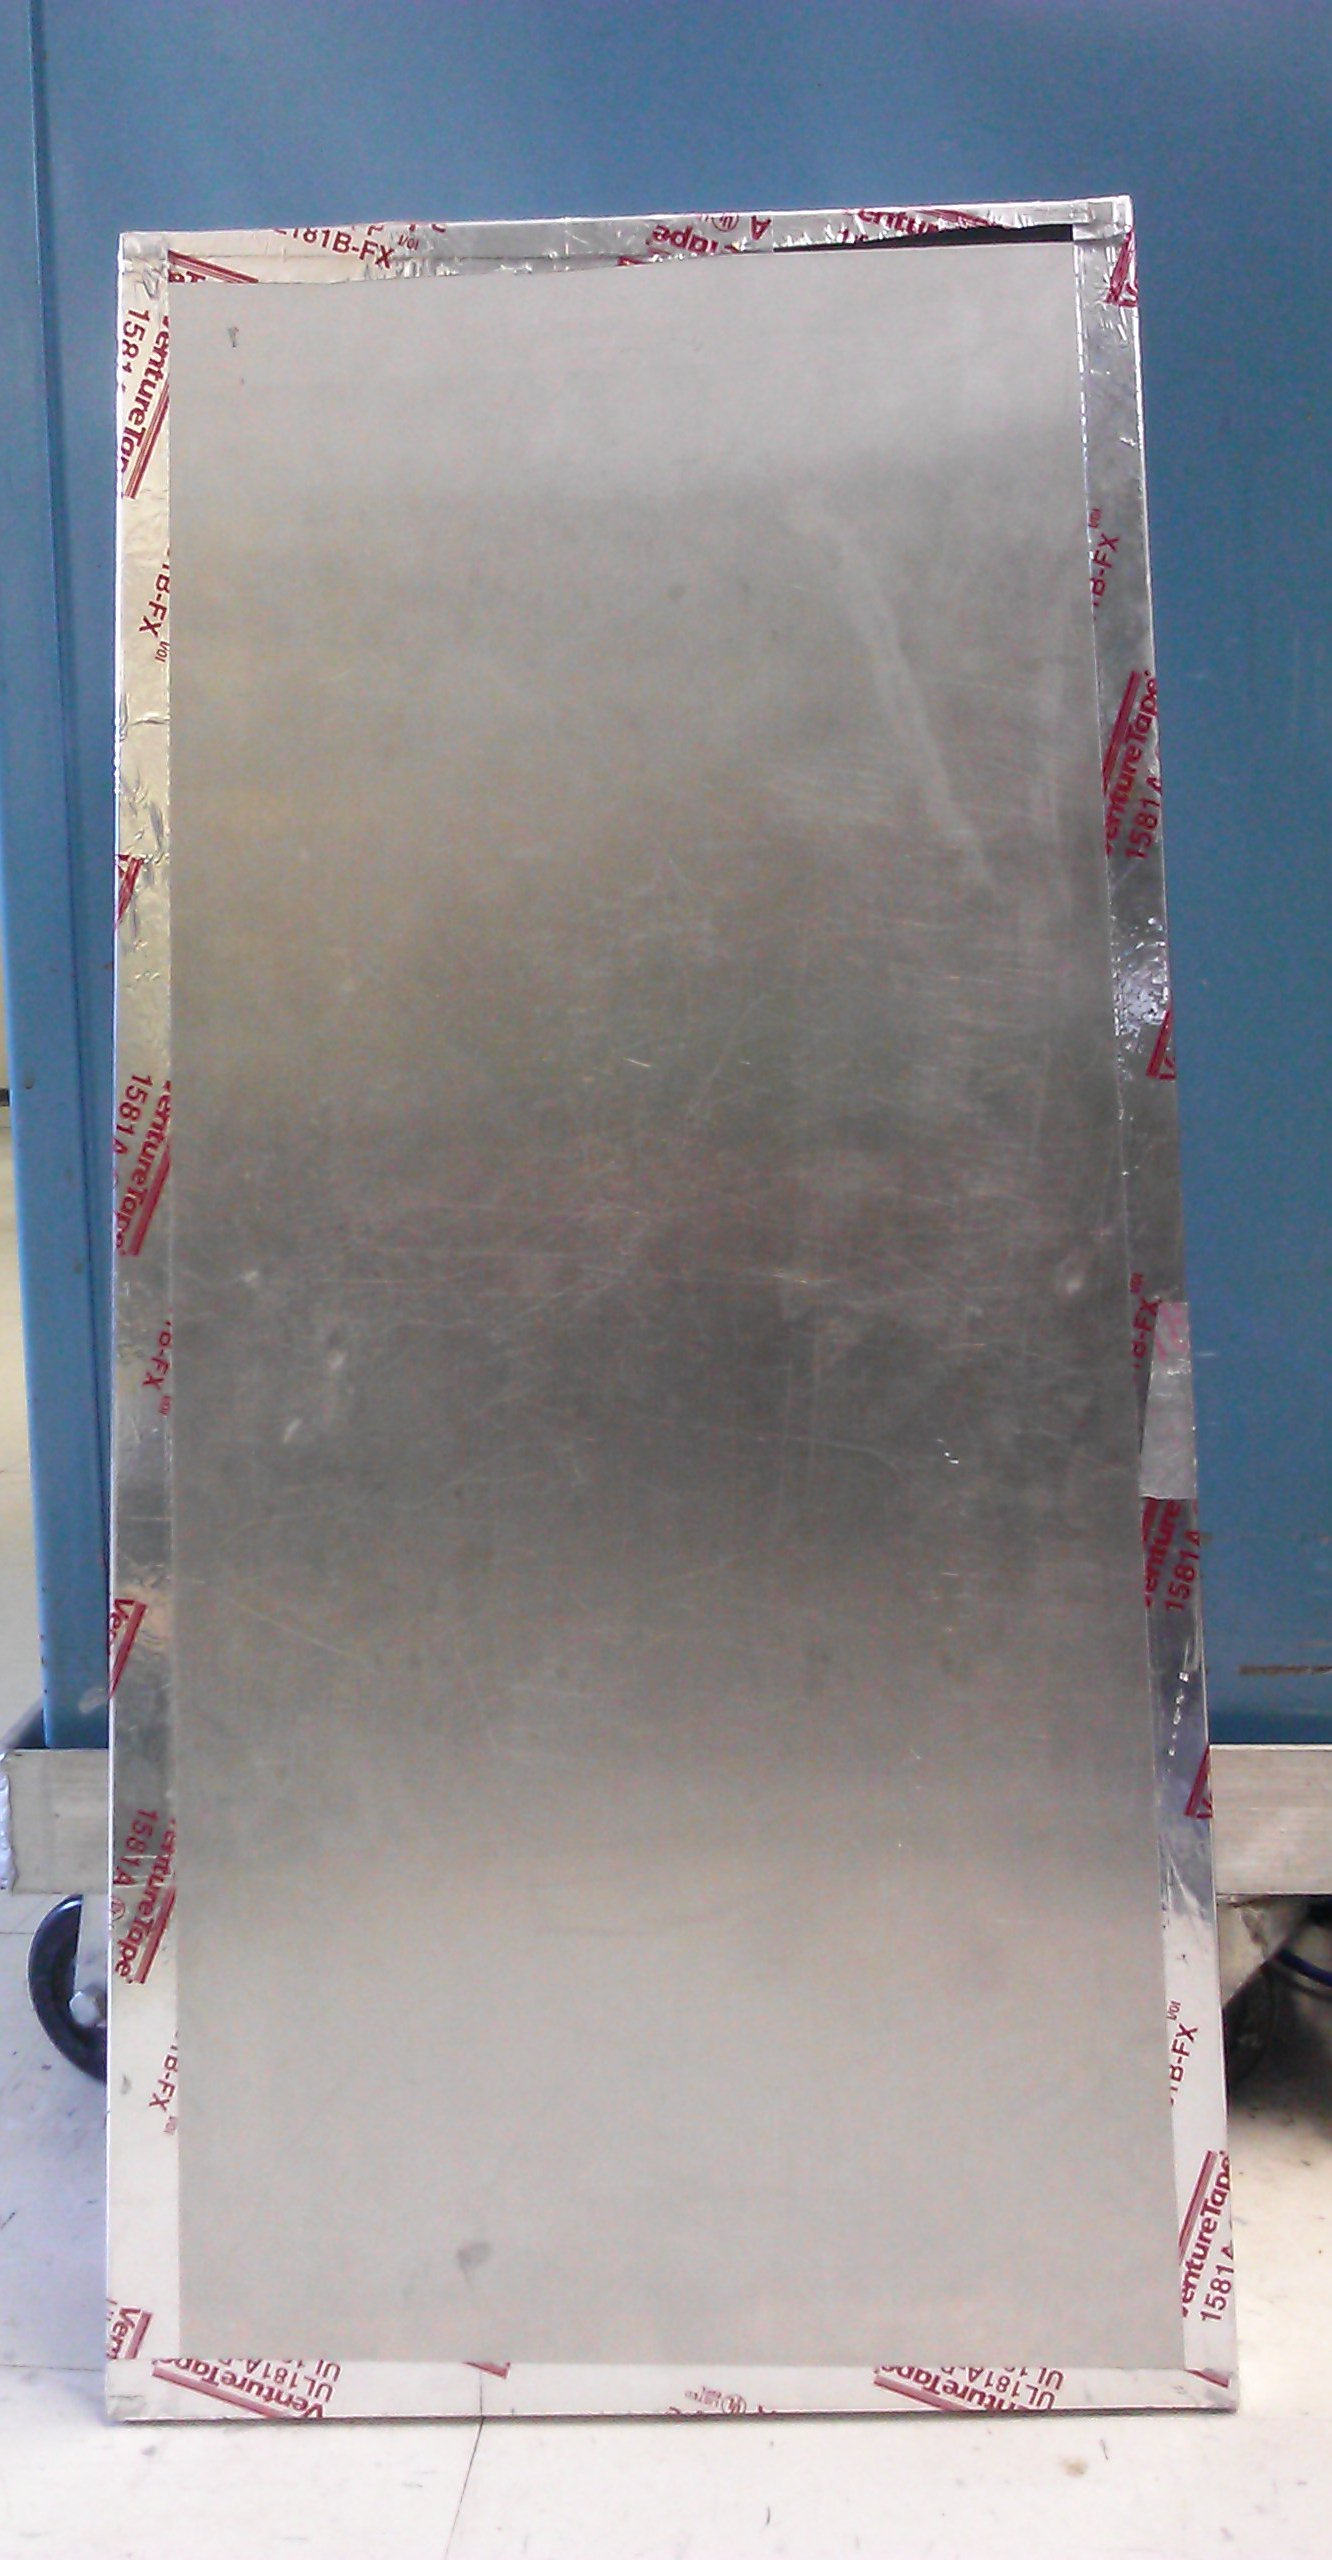
\includegraphics[angle=90,width=0.7\textwidth]{figures/Cosmic_Paddle.jpg}
\caption{
Photograph of one of the scintillation counters used in the cosmic towers. 
} 
\label{pic:cosmicpaddle}
\end{figure}

The paddles were selected from a pool of over 300 scintillating counters collected during the decommissioning of the CDF detector at Fermilab. 
For each counter, both the efficiency $\varepsilon_P$ and the noise $\eta_P$ as a function of the voltage were determined. The measurement was performed sandwiching the given paddle among 4 sample counters, placed two above and two below the paddle under test. The efficiency 
$\varepsilon_P$ was defined as the ratio between the 5-fold coincidence and the 4-fold coincidence of the sample counters. The accidental rate $\eta_P$ was instead defined as the number of 5-fold coincidence observed during ten minutes of data acquisition, when the signal of the paddle under test was delayed by $5 \mu s$. Each paddle with $\varepsilon_P \geq 95\%$ and $\eta_P = 0$ at working voltage was identified as a candidate for the Cosmic Ray system. The ones with the highest efficiency and lowest single count rate were then selected to realize the system itself. 
The plot of $\varepsilon_P$ as a function of the PMT voltage for one example paddle is shown in Fig. \ref{pic:CR_Effplot}.

\begin{figure}[h!]
 \centering
% \includegraphics[width=0.7\textwidth]{figures/TSU29_Efficiency.png}
\caption{
Plot of the counter efficiency $\varepsilon_P$ as a function of the PMT voltage for one of the paddles composing the Cosmic Ray system. 
} 
\label{pic:CR_Effplot}
\end{figure}


%$\varepsilon_P$ at a given voltage is defined as:

%$$
%\varepsilon_P = \frac{R_{1-2} \land R_{3-4} \land R_P}{R_{1-2} \land R_{3-4}}
%$$

%where $R_P$ is the rate of the paddle $P$ to be tested, $R_{1-2}$ is the coincidence rate of two sample paddles positioned above $P$, while $R_{3-4}$ is the coincidence rate of two sample paddles positioned below $P$.
%$\eta_P$ at a given voltage is instead defined as:

%$$
%\eta_P = \frac{R_{1-2} \land R_{3-4} \land R_{P^*}}{R_{1-2} \land R_{3-4}}
%$$

%where $R_{P^*}$ is the Rate of the paddle $P$ 


The trigger rate $R$ of the whole system is $R=0.032Hz$, corresponding to $\sim 1.9~\mu/minute$.
\end{comment}

